\documentclass{article}
\usepackage[utf8]{inputenc}
\usepackage{amsmath}
\usepackage{graphicx}
\usepackage{longtable}
\usepackage{geometry}
\usepackage{array}
\usepackage{hyperref}
\usepackage{enumitem}
\usepackage{xcolor}
\usepackage{listings}
\usepackage{fancyhdr}
\usepackage{float}
\usepackage{tikz}
\usetikzlibrary{automata,positioning}

\geometry{a4paper, margin=1in}
\hypersetup{colorlinks=true, urlcolor=blue}

% Define a custom command for roles
\newcommand{\role}[1]{\textbf{\textcolor{blue}{#1:}}}

% Setup for code listings
\lstset{
    backgroundcolor=\color{lightgray!20},
    basicstyle=\footnotesize\ttfamily,
    breaklines=true,
    frame=single,
    rulecolor=\color{black},
    showstringspaces=false,
    tabsize=2
}

\pagestyle{fancy}
\fancyhf{}
\fancyhead[L]{Library Management System Testing Guide}
\fancyfoot[C]{\thepage}

\title{Comprehensive Testing Guide for the Library Management System}
\author{SE507 Group Project - Spring 2025}
\date{\today}

\begin{document}

\maketitle

\begin{abstract}
This document provides a complete guide for testing the Library Management System, based on the Software Requirements Specification (SRS) and the established project tasks. It is designed to be used by both technical and non-technical team members, providing clear instructions and best practices for each phase of the testing lifecycle. The guide leverages modern technologies and methodologies discussed in the course lectures to ensure a high-quality, robust, and reliable final product.
\end{abstract}

\section{Introduction}

The Library Management System is a comprehensive software solution designed to automate and streamline the operations of a library. The successful implementation of this system relies on a rigorous and well-structured testing process. This guide is based on the provided project files, including the SRS, task distribution documents, and course lectures. It aims to provide a unified framework for all testing activities.

\subsection{Purpose and Scope}
The primary purpose of this guide is to detail the methodologies, tools, and best practices for testing the Library Management System. The scope encompasses all phases of testing, from initial static analysis to final user acceptance testing, ensuring that all functional and non-functional requirements outlined in the SRS are met.

\subsection{Team Composition and Responsibilities}
The testing team is composed of members with diverse skill sets, categorized as follows:
\begin{itemize}
    \item \textbf{Coders:} Team members with strong programming and technical skills. They are primarily responsible for white-box testing, automation, and performance analysis.
    \item \textbf{Non-Coders/Specification Experts:} Team members who excel at user-centric evaluation and requirements analysis. They are responsible for black-box testing, usability testing, and ensuring the system aligns with user expectations.
\end{itemize}
A detailed breakdown of task distribution is provided in the "Task Distribution for Library Management Project Testing.docx" document and is summarized in the relevant sections of this guide.

\section{Testing Strategy}

The testing strategy is designed to be comprehensive, covering all aspects of the system. It integrates various testing levels and types to ensure maximum defect detection and quality assurance.

\subsection{Testing Levels}
The project will follow a standard V-Model approach to testing, with the following levels:
\begin{itemize}
    \item \textbf{Unit Testing:} (Primarily performed by developers) To test individual components in isolation.
    \item \textbf{Integration Testing:} To test the interfaces and interactions between integrated components.
    \item \textbf{System Testing:} To test the complete, integrated system against the SRS.
    \item \textbf{Acceptance Testing:} To validate the system from a user's perspective.
\end{itemize}

\subsection{Testing Types}
Both functional and non-functional testing will be performed:
\begin{itemize}
    \item \textbf{Functional Testing:} Validates the software against the functional requirements. This includes:
    \begin{itemize}
        \item Use Case Testing
        \item State Transition Testing
        \item Entity Management Testing
        \item Authentication and Authorization Testing
    \end{itemize}
    \item \textbf{API Testing:} Focuses on testing the Application Programming Interfaces (APIs) directly.
    \item \textbf{Non-Functional Testing:} Validates aspects of the system not related to specific functions. This includes:
    \begin{itemize}
        \item Performance Testing
        \item Security Testing
        \item Usability Testing
        \item Browser Compatibility Testing
        \item Maintainability Testing
    \end{itemize}
    \item \textbf{Regression Testing:} To ensure that new changes do not negatively impact existing functionality.
    \item \textbf{Static Testing:} Involves reviewing code and documentation without executing the software.
\end{itemize}

\section{Technological Stack and Tools}

The project utilizes a modern technology stack that requires specific tools for effective testing.

\subsection{Application Stack}
\begin{itemize}
    \item \textbf{Frontend:} React.js
    \item \textbf{Backend:} Node.js with Express.js
    \item \textbf{Database:} MongoDB
    \item \textbf{Containerization:} Docker
\end{itemize}

\subsection{Testing Tools}
\begin{itemize}
    \item \textbf{API Testing:} Postman will be used for manual and automated API testing.
    \item \textbf{End-to-End Testing:} Cypress is the designated tool for automated end-to-end testing.
    \item \textbf{Performance Testing:} Tools like JMeter or k6 can be used to simulate load and measure performance.
    \item \textbf{Code Analysis:} Linters and static analysis tools integrated into the development environment.
\end{itemize}


\subsection{Environment Setup}
Before any testing can begin, the application environment must be running.

\role{Coders}
Your primary responsibility is to manage the Docker environment.
\begin{enumerate}
    \item \textbf{Navigate to Root Directory:} Open a terminal in the project's root folder.
    \item \textbf{Build and Run Containers:} Execute the command:
    \begin{lstlisting}[language=bash]
docker-compose -f docker-compose.dev.yml up --build
    \end{lstlisting}
    This command starts the frontend, backend, and database services as defined in the development compose file.
    \item \textbf{Verify Services:}
    \begin{itemize}
        \item The React frontend should be accessible at \href{http://localhost:3000}{\texttt{http://localhost:3000}}.
        \item The Node.js backend API will be running on \href{http://localhost:5000}{\texttt{http://localhost:5000}}.
    \end{itemize}
    \item \textbf{Troubleshooting:} If containers fail to start, check the Docker logs for errors. Common issues include port conflicts or configuration errors in the `.yml` files.
\end{enumerate}

\role{Non-Coders}
Your main setup task is to ensure you can access the application and have the necessary tools ready.
\begin{enumerate}
    \item \textbf{Access the Application:} Once the Coders have confirmed the environment is up, open a web browser and navigate to \href{http://localhost:3000}{\texttt{http://localhost:3000}}.
    \item \textbf{Install Postman:} If you don't have it, download and install Postman. This will be your primary tool for API testing.
\end{enumerate}

\section{Static Testing (Non-Execution Based)}
Static testing is performed early in the lifecycle to find defects without executing code. It involves reviewing documentation and source code.

\subsection{Documentation Review}
\role{Non-Coders/Specification Experts}
You will lead the review of all non-technical and requirements-related documents.
\begin{itemize}
    \item \textbf{Source Documents:} ``SRS Library Management.docx'', ``Tasks.pdf'', all ``TC\_*.tex'' files.
    \item \textbf{Objective:} Check for clarity, consistency, completeness, and correctness. Ensure the test cases accurately reflect the requirements in the SRS.
    \item \textbf{Process:} Read through the documents, noting any ambiguities, contradictions, or missing information. Use a collaborative document or a simple spreadsheet to log your findings.
\end{itemize}

\role{Coders}
You will support the documentation review by focusing on technical accuracy.
\begin{itemize}
    \item \textbf{Objective:} Review the SRS and test plans to ensure they are technically feasible and that the descriptions of system behavior are accurate from an implementation perspective.
    \item \textbf{Process:} Participate in review meetings led by the Non-Coders and provide feedback on technical sections.
\end{itemize}

\subsection{Code Review}
\role{Coders}
You will lead the technical review of the source code.
\begin{itemize}
    \item \textbf{Source Files:} All `.js`, `.jsx`, and `.ts` files in the `client/`, `server/`, and `e2e/` directories.
    \item \textbf{Objective:} Identify potential bugs, security vulnerabilities, and deviations from coding standards. Assess logic, efficiency, and maintainability.
    \item \textbf{Process:} Use a systematic approach. For example, for each file, check:
    \begin{enumerate}
        \item Is the logic correct and efficient?
        \item Is there proper error handling?
        \item Are there any obvious security flaws (e.g., hardcoded secrets, injection vulnerabilities)?
        \item Does the code adhere to project-wide standards for naming and style?
    \end{enumerate}
\end{itemize}

\role{Non-Coders/Specification Experts}
Your role is to ensure the code is understandable and aligns with the specified requirements.
\begin{itemize}
    \item \textbf{Objective:} Focus on readability, comments, and the high-level structure of the code. You are not expected to understand complex algorithms, but rather to assess if the code's purpose is clear and seems to match the user stories.
    \item \textbf{Process:} During review sessions (or "walkthroughs") led by the Coders, ask questions to clarify how the code achieves a specific feature described in the SRS. For example: "Can you show me the code that prevents a non-librarian from adding a book?"
\end{itemize}


\section{Functional and API Testing}
This phase focuses on verifying that the system behaves according to its specifications.

\subsection{API Testing with Postman}
\role{Non-Coders/Specification Experts}
Your primary role is to design the test scenarios based on the SRS.
\begin{enumerate}
    \item \textbf{Document Reference:} \texttt{TC\_API\_Testing.tex}.
    \item \textbf{Task:} For each API endpoint (e.g., `POST /api/auth/login`, `GET /api/book/getAll`), define test cases for:
    \begin{itemize}
        \item \textbf{Positive scenarios:} Testing with valid data (e.g., logging in with correct credentials).
        \item \textbf{Negative scenarios:} Testing with invalid data (e.g., logging in with a wrong password, trying to fetch a book with an invalid ID).
        \item \textbf{Edge cases:} Testing boundary conditions (e.g., empty request bodies, very long strings).
    \end{itemize}
    \item \textbf{Execution:} Using Postman, you will manually execute these scenarios. For a `POST` request, you will set the URL, select the method, and provide the JSON body. After sending the request, verify that the HTTP status code (e.g., 200, 401, 404) and the response body match your expected results.
\end{enumerate}

\role{Coders}
Your role is to automate the scenarios designed by the Non-Coders and to test more complex API interactions.
\begin{enumerate}
    \item \textbf{Task:} Use Postman's test scripting features (or a framework like `supertest` as seen in `auth.api.test.js`) to create automated test suites.
    \item \textbf{Example Postman Test Script:} For the login endpoint, you can write a test to verify the response:
    \begin{lstlisting}[language=Java]
pm.test("Status code is 200", function () {
    pm.response.to.have.status(200);
});
pm.test("Response contains an authentication token", function () {
    var jsonData = pm.response.json();
    pm.expect(jsonData.token).to.not.be.empty;
});
    \end{lstlisting}
    \item \textbf{Chained Requests:} Create tests that chain requests together. For example, a test could first log in to get a token, then use that token in the header of a subsequent request to access a protected endpoint.
\end{enumerate}

\subsection{End-to-End (E2E) Testing with Cypress}
E2E testing simulates real user scenarios from start to finish.

\role{Coders}
You are responsible for writing and maintaining the Cypress E2E tests.
\begin{enumerate}
    \item \textbf{Source Files:} The primary files are in the `e2e/cypress/e2e/` directory, such as `authentication\_authorization.cy.ts`.
    \item \textbf{Running Tests:}
    \begin{itemize}
        \item \textbf{Interactive Mode:} Use this for writing and debugging tests.
        \begin{lstlisting}[language=bash]
# From the root directory
npm run e2e:watch
        \end{lstlisting}
        \item \textbf{Headless Mode:} Use this for running the full test suite (e.g., in a CI/CD pipeline).
        \begin{lstlisting}[language=bash]
# From the root directory
npm run e2e
        \end{lstlisting}
    \end{itemize}
    \item \textbf{Writing Tests:} Follow the existing patterns in `authentication\_authorization.cy.ts`. Use descriptive `describe` and `it` blocks. Use commands like `cy.visit()`, `cy.get()`, `cy.click()`, and `cy.type()` to interact with the UI. Use assertions like `.should('exist')` or `.should('contain', 'text')` to verify outcomes.
\end{enumerate}

\role{Non-Coders/Specification Experts}
You are responsible for designing the E2E test scenarios and validating the results.
\begin{enumerate}
    \item \textbf{Task:} Based on the Use Cases in the SRS (e.g., `UC-002: Add New Book`), write out the step-by-step user actions and expected outcomes in plain language.
    \item \textbf{Example Scenario (Add New Book):}
    \begin{enumerate}
        \item Login as a Librarian.
        \item Navigate to the "Book Management" page.
        \item Click the "Add Book" button.
        \item Fill in the book title, author, genre, and other details in the form.
        \item Click "Save".
        \item \textbf{Expected Result:} The new book appears in the list on the "Book Management" page. A success notification is shown.
    \end{enumerate}
    \item \textbf{Collaboration:} Provide these scenarios to the Coders to be automated. You will then review the execution of the automated tests (either by watching them run or by checking the reports) to confirm they match the intended user flow.
\end{enumerate}

\section{Non-Functional Testing}
This phase tests system attributes like performance, security, and usability.

\subsection{Usability Testing}
\role{Non-Coders/Specification Experts}
You will lead usability testing, as it is entirely user-focused.
\begin{itemize}
    \item \textbf{Document Reference:} `TC\_Usability\_Testing.tex`.
    \item \textbf{Objective:} Evaluate how easy and intuitive the system is to use.
    \item \textbf{Process (Heuristic Evaluation):} Go through the application and assess it against established usability principles:
    \begin{itemize}
        \item \textbf{Consistency:} Are buttons, menus, and terminology consistent across all pages?
        \item \textbf{Feedback:} Does the system provide clear feedback for actions (e.g., showing a "loading" spinner, a "success" message)?
        \item \textbf{Clarity:} Is the text clear and unambiguous? Are icons easy to understand?
        \item \textbf{Error Prevention:} Is it easy for users to make mistakes? How does the system help prevent them?
    \end{itemize}
    \item \textbf{Reporting:} Document findings with screenshots and detailed descriptions of any confusing or difficult-to-use parts of the interface.
\end{itemize}

\subsection{Security Testing}
\role{Coders}
You are responsible for technical security testing.
\begin{itemize}
    \item \textbf{Document Reference:} `TC\_Security\_Testing.tex`.
    \item \textbf{Key Areas to Test:}
    \begin{itemize}
        \item \textbf{Authorization Bypass:} Use Postman to try accessing a librarian-only API endpoint (e.g., `POST /api/book/add`) using the authentication token of a regular member. The expected result is a `403 Forbidden` status code.
        \item \textbf{Data Exposure:} Check the responses of all API endpoints to ensure they are not leaking sensitive information (e.g., the user list endpoint should not return password hashes).
    \end{itemize}
\end{itemize}

\subsection{Performance Testing}
\role{Coders}
You will lead performance testing using appropriate tools.
\begin{itemize}
    \item \textbf{Document Reference:} `TC\_Performance\_Testing.tex`.
    \item \textbf{Tool:} Apache JMeter or k6.
    \item \textbf{Objective:} Determine how the system behaves under load.
    \item \textbf{Process (Load Test):}
    \begin{enumerate}
        \item Create a test plan in JMeter.
        \item Define a Thread Group to simulate a number of concurrent users (e.g., 50 users).
        \item Add HTTP Request samplers for key API endpoints (e.g., `GET /api/book/getAll`).
        \item Add listeners to view the results (e.g., Summary Report, Aggregate Graph).
        \item Run the test and analyze the results, focusing on average response time and error rate. The system should maintain acceptable response times without a high error percentage.
    \end{enumerate}
\end{itemize}

\section{Regression Testing}
Regression testing is crucial to ensure that new features or bug fixes have not broken existing functionality.

\role{Coders}
You are responsible for running the automated regression suite.
\begin{itemize}
    \item \textbf{Process:} After any significant code change, run the entire Cypress E2E test suite and the automated Postman/API test suite.
    \item \textbf{Objective:} All tests should pass. Any failures indicate a regression that must be fixed before the changes are accepted.
\end{itemize}

\role{Non-Coders/Specification Experts}
You are responsible for performing manual, risk-based regression testing.
\begin{itemize}
    \item \textbf{Document Reference:} `TC\_Regression\_Testing.tex`.
    \item \textbf{Process:} Based on the recent changes, identify the areas of the application most at risk. For example, if a change was made to the borrowing logic, you should manually re-test:
    \begin{itemize}
        \item Borrowing a book.
        \item Trying to borrow an already borrowed book.
        \item Viewing borrowal history.
        \item Returning a book.
    \end{itemize}
    \item \textbf{Objective:} To provide an additional layer of confidence by testing scenarios that may not be covered by automation.
\end{itemize}

\section{Advanced Functional Testing Scenarios}
This section expands on the core functional testing by introducing model-based techniques and a deeper focus on data integrity, as discussed in the lectures.

\subsection{Entity Management and Data Integrity Testing}
This testing ensures that the relationships between data entities (Books, Authors, etc.) are correctly enforced by the system.

\role{Non-Coders/Specification Experts}
You are responsible for designing the test cases based on the data model in the SRS.
\begin{itemize}
    \item \textbf{Document Reference:} `TC\_Entity\_Management.tex`.
    \item \textbf{Objective:} To verify that all Create, Read, Update, and Delete (CRUD) operations work as expected and that data constraints are enforced.
    \item \textbf{Task:} For each entity, design tests for scenarios like:
    \begin{itemize}
        \item Attempting to create a `Book` without selecting a valid `Author` or `Genre`. The system should show an error.
        \item Attempting to delete an `Author` who still has `Book`s associated with them in the system. This should be prevented.
        \item Updating a `User`'s role and verifying their permissions change accordingly.
    \end{itemize}
    \item \textbf{Execution:} These tests are typically run manually through the UI, checking that the system behaves as you've designed.
\end{itemize}

\subsection{State Transition Testing}
As covered in the lectures, systems can often be modeled as a Finite State Machine (FSM). This technique tests the transitions between different states of an entity. The `Borrowal` entity is a perfect candidate.

\role{Non-Coders/Specification Experts}
Your role is to model the entity's lifecycle and design tests to cover it.
\begin{itemize}
    \item \textbf{Document Reference:} `TC\_State\_Transition\_Testing.tex`.
    \item \textbf{Modeling:} First, define the states and transitions for a borrowal.
    
    \begin{center}
    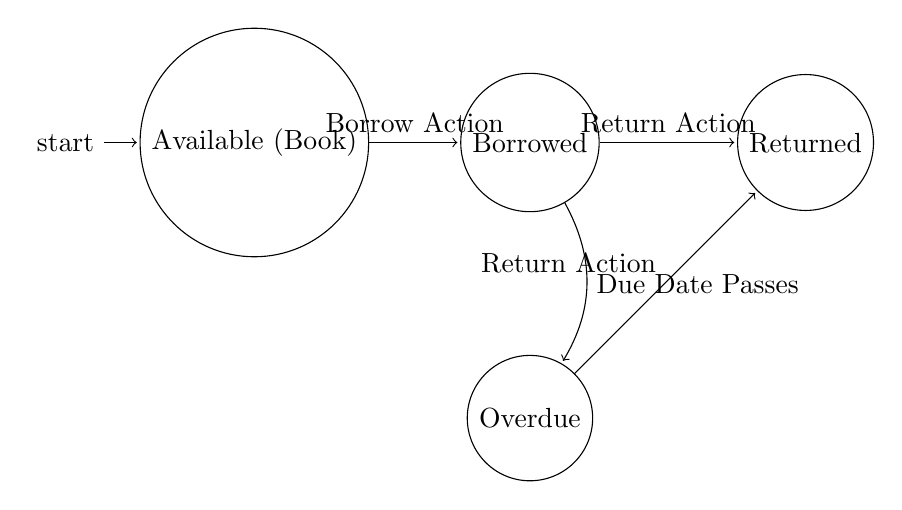
\begin{tikzpicture}[shorten >=1pt,node distance=3.5cm,on grid,auto] 
       \node[state,initial] (A) {Available (Book)};
       \node[state] (B) [right=of A] {Borrowed};
       \node[state] (C) [right=of B] {Returned};
       \node[state] (D) [below=of B] {Overdue};
        \path[->] 
        (A) edge node {Borrow Action} (B)
        (B) edge node {Return Action} (C)
        (B) edge [bend left] node {Due Date Passes} (D)
        (D) edge node {Return Action} (C);
    \end{tikzpicture}
    \end{center}
    
    \item \textbf{Test Design:} Create test cases that trigger each transition. For example:
    \begin{itemize}
        \item \textbf{Test 1 (A to B):} Log in as a member, find an available book, and execute the borrow function. Verify the book's status changes to "Borrowed".
        \item \textbf{Test 2 (B to D):} For a borrowed book, manually change the system date past the due date (a Coder may need to assist with this) and verify the status becomes "Overdue".
        \item \textbf{Test 3 (Invalid Transition):} Attempt to borrow an already "Borrowed" book. The system should display an error.
    \end{itemize}
\end{itemize}

\role{Coders}
Your task is to automate these state transition tests where feasible.
\begin{itemize}
    \item \textbf{Objective:} To create robust tests that can programmatically drive an entity through its lifecycle.
    \item \textbf{Process:} This often requires a combination of API calls. For the borrowal example, an automated test script could:
    \begin{enumerate}
        \item Call the login API to get a member token.
        \item Call the `borrow` API endpoint.
        \item Call a special debug endpoint (that you might create) to advance the time on the server.
        \item Call the `getBorrowal` API to check that the status is now 'Overdue'.
        \item Call the `return` API.
        \item Call `getBorrowal` again to check that the status is 'Returned'.
    \end{enumerate}
\end{itemize}


\section{Integration Testing}
Integration testing focuses on verifying the interaction between different components or modules of the system.

\role{Coders}
You will lead the implementation of integration tests, as they are primarily code-based.
\begin{itemize}
    \item \textbf{Document Reference:} `TC\_Integration\_Testing.tex` and the existing test `server/\_\_tests\_\_/integration/auth.api.test.js`.
    \item \textbf{Objective:} Test the data flow and communication between the Node.js backend API and the MongoDB database.
    \item \textbf{Process:} Write tests using a framework like `supertest` and `jest`. These tests make real API calls to the server and can check the database state to verify the outcome.
    \item \textbf{Example Integration Test Scenario:}
    \begin{enumerate}
        \item The test starts by clearing the relevant database collections.
        \item It makes a `POST /api/author/add` request to create a new author.
        \item It then directly queries the database to assert that the author document was created correctly.
        \item It makes a `POST /api/book/add` request, using the new author's ID.
        \item It queries the database to assert that the book was created and correctly references the author.
    \end{enumerate}
\end{itemize}

\role{Non-Coders/Specification Experts}
You will support integration testing by defining the cross-module user workflows.
\begin{itemize}
    \item \textbf{Task:} Identify user journeys that touch multiple parts of the system.
    \item \textbf{Example Scenario:} "A member searches for a book, finds it, adds a review for it, and then borrows it. This workflow integrates the Search, Review, and Borrowal modules."
    \item \textbf{Collaboration:} Provide these high-level scenarios to the Coders to guide the creation of their technical integration tests.
\end{itemize}


\section{Finalizing the Testing Process}

\subsection{Browser Compatibility Testing}
\role{Non-Coders/Specification Experts}
You will lead the manual execution of these tests.
\begin{itemize}
    \item \textbf{Document Reference:} `TC\_Browser\_Compatibility\_Testing.tex`.
    \item \textbf{Objective:} To ensure the application looks and works correctly on major web browsers.
    \item \textbf{Process:}
    \begin{enumerate}
        \item Identify the target browsers (e.g., latest versions of Chrome, Firefox, and Safari/Edge).
        \item Execute a set of key test cases (a "smoke test" suite) on each browser. This should include core functionality like login, search, and viewing data tables.
        \item Look for any visual bugs (e.g., misaligned elements, broken layouts) or functional issues (e.g., buttons not working).
        \item Document any differences in behavior with screenshots.
    \end{enumerate}
\end{itemize}

\subsection{Defect Management and Reporting}
A structured approach to managing defects is essential for project success.

\role{Both Coders and Non-Coders}
Defect reporting is a shared responsibility.
\begin{enumerate}
    \item \textbf{Finding a Defect:} When a test case fails (either manual or automated), a defect has been found.
    \item \textbf{Logging the Defect:} Create a defect report using a simple tool (like a shared spreadsheet, Trello, or Jira). The report MUST contain:
    \begin{itemize}
        \item[--] A clear, concise title (e.g., "Login fails with valid member credentials").
        \item[--] The environment it was found in (e.g., Local dev, Chrome).
        \item[--] Detailed, numbered steps to reproduce the bug.
        \item[--] The \textbf{Expected Result} (what should have happened).
        \item[--] The \textbf{Actual Result} (what did happen).
        \item[--] Screenshots or log files.
        \item[--] An initial assessment of Severity (how much impact it has on the system) and Priority (how urgently it should be fixed).
    \end{itemize}
\end{enumerate}

\role{Coders}
You are responsible for resolving defects.
\begin{enumerate}
    \item Pick up a defect from the log.
    \item Analyze the issue and implement a code fix.
    \item Update the defect report, marking it as "Ready for Retest".
\end{enumerate}

\role{Non-Coders/Specification Experts}
You are responsible for verifying fixes.
\begin{enumerate}
    \item Take a defect marked "Ready for Retest".
    \item Execute the original test case that found the bug.
    \item If the bug is gone, close the defect report. If it still exists, re-open it and assign it back to the Coders with a comment.
\end{enumerate}

\section{Maintainability Testing}
Maintainability testing assesses the ease with which the system can be understood, modified, and enhanced. This is a crucial non-functional requirement for the long-term health of the project.

\role{Coders}
You are responsible for the technical analysis of the codebase's maintainability.
\begin{itemize}
    \item \textbf{Document Reference:} `TC\_Maintainability.tex`.
    \item \textbf{Objective:} To measure the structural quality and complexity of the code.
    \item \textbf{Key Metrics and Tools:}
    \begin{itemize}
        \item \textbf{Code Coverage:} Use the built-in Jest test coverage reporting. After running tests, check the coverage report. A higher percentage indicates that more code is exercised by tests, making it safer to modify.
        \begin{lstlisting}[language=bash]
# From the /server directory
npm test -- --coverage
        \end{lstlisting}
        \item \textbf{Code Complexity:} Manually assess the cyclomatic complexity of critical functions (e.g., in `borrowalController.js`). A function with many nested `if`/`else` statements or loops has high complexity and is harder to maintain. Aim to refactor highly complex functions into smaller, simpler ones.
        \item \textbf{Static Analysis:} Pay close attention to warnings from ESLint. These tools are designed to catch "code smells" that can indicate poor maintainability.
    \end{itemize}
\end{itemize}

\role{Non-Coders/Specification Experts}
You will assess maintainability from a documentation and knowledge transfer perspective.
\begin{itemize}
    \item \textbf{Objective:} To evaluate how easy it would be for a new team member to understand the system.
    \item \textbf{Process:}
    \begin{itemize}
        \item \textbf{Documentation Quality:} Review the code comments, the `README.md` files, and the SRS. Is the documentation clear, accurate, and up-to-date?
        \item \textbf{Traceability:} Can you trace a requirement from the SRS to a specific test case and, with a Coder's help, to the part of the code that implements it? Strong traceability is a sign of a maintainable system.
        \item \textbf{Configuration Management:} Review the `docker-compose` files. Are the configurations easy to understand? Is it clear how to start the system in different environments (dev, test, prod)?
    \end{itemize}
\end{itemize}

\section{Test Metrics and Exit Criteria}
To manage the testing process effectively and to know when to stop, the team must define and track key metrics and agree on "exit criteria".

\subsection{Key Performance Indicators (KPIs) for Testing}
\role{Both Coders and Non-Coders}
The entire team is responsible for tracking and discussing these metrics in regular meetings. A simple shared spreadsheet can be used as a dashboard.

\begin{itemize}
    \item \textbf{Requirements Coverage:} What percentage of requirements defined in the SRS have at least one test case associated with them? The goal is 100\%.
    \item \textbf{Test Case Pass Rate:} The percentage of executed test cases that have passed.
    $$ \text{Pass Rate} = \left( \frac{\text{Number of Passed Tests}}{\text{Total Number of Executed Tests}} \right) \times 100\% $$
    \item \textbf{Defect Density:} The number of confirmed defects per module or feature. This helps identify which parts of the application are most unstable.
    \item \textbf{Defect Discovery Rate (DDR):} The number of defects found per day or week. A falling DDR towards the end of the cycle can indicate that the system is stabilizing.
\end{itemize}

\subsection{Test Exit Criteria}
These are the conditions that must be met for the team to formally conclude the testing phase.
\begin{itemize}
    \item A Test Case Pass Rate of at least \textbf{95\%} has been achieved.
    \item Requirements Coverage is \textbf{100\%}.
    \item All automated E2E and Integration test suites run to completion with \textbf{100\%} of tests passing.
    \item There are \textbf{zero} open defects with a "Blocker" or "Critical" severity level.
    \item All "High" severity defects have a documented plan for being fixed, or a formal decision has been made to accept the risk.
    \item The Final Test Summary Report has been reviewed and approved by the entire team.
\end{itemize}

\section{Final Test Summary Report}
This is the final document produced by the testing team. It provides a comprehensive overview of all testing activities and gives a final assessment of the software's quality.

\role{Non-Coders/Specification Experts}
You will lead the compilation of this report, with Coders contributing to the technical sections.

\subsection{Structure of the Report}
The report should contain the following sections:
\begin{enumerate}
    \item \textbf{Introduction:} A brief overview of the project and the scope of the testing conducted.
    \item \textbf{Testing Scope and Approach:} A summary of the testing types performed (Functional, API, Performance, etc.) and the tools used.
    \item \textbf{Test Results and Metrics:}
        \begin{itemize}
            \item A summary of the final test metrics (Requirements Coverage, Pass Rate, etc.).
            \item A summary of the results for each type of testing performed. For example, a section on Performance Testing should state the average response times under load.
        \end{itemize}
    \item \textbf{Defect Summary:}
        \begin{itemize}
            \item An overview of the total number of defects found, categorized by severity (Blocker, Critical, High, Medium, Low).
            \item A list of any critical or high-severity defects that are still open, along with a justification if they are not being fixed.
        \end{itemize}
    \item \textbf{Overall Quality Assessment:} The team's final, professional judgment on the quality of the system. This section should explicitly state whether the system meets the quality goals defined at the start of the project.
    \item \textbf{Recommendation:} A clear recommendation on whether the software is ready for "release" (i.e., project submission) based on the test results and exit criteria.
    \item \textbf{Lessons Learned:} A brief section detailing what went well in the testing process and what could be improved in future projects.
\end{enumerate}

\appendix
\section{Appendix: Quick Reference}

\subsection{Key Commands}
\begin{description}
    \item[Run Dev Environment:] \texttt{docker-compose -f docker-compose.dev.yml up --build}
    \item[Run Cypress (Interactive):] \texttt{npm run e2e:watch}
    \item[Run Cypress (Headless):] \texttt{npm run e2e}
    \item[Run Backend Tests:] \texttt{cd server \&\& npm test}
\end{description}

\subsection{Glossary of Terms}
\begin{description}
    \item[Black-Box Testing:] Testing a system without knowledge of its internal workings.
    \item[White-Box Testing:] Testing based on knowledge of the internal logic of an application's code.
    \item[Regression Testing:] Re-running functional and non-functional tests to ensure that previously developed and tested software still performs after a change.
    \item[State Transition Testing:] A black-box technique used to test the behavior of a system as it moves between different states.
    \item[SRS:] Software Requirements Specification.
\end{description}


\end{document}
